%Titre
\section{La transformée de Fourier}

%%%%%%%%%%%%%%%%%%%%%%%%%%%%%%%%%%%%%%%%%%%%%%%%
% Première diapo
%%%%%%%%%%%%%%%%%%%%%%%%%%%%%%%%%%%%%%%%%%%%%%%%
\begin{frame}{La transformée de Fourier}{}
    \begin{block}{Definition}
        La transformée de Fourier est un opérateur, qui permet de transformer un signal sous forme temporelle en signal sous forme fréquentielle: 
         \[ \forall f \in L^1 \, \forall x \in \mathbb{R} \; \mathcal{F}(f)(x) = \int_{-\infty}^{+\infty} f(t)e^{-2i\pi xt}\mathrm{d}t\]
    \end{block}
\end{frame}

%%%%%%%%%%%%%%%%%%%%%%%%%%%%%%%%%%%%%%%%%%%%%%%%
% Deuxième diapo
%%%%%%%%%%%%%%%%%%%%%%%%%%%%%%%%%%%%%%%%%%%%%%%%
\begin{frame}{La transformée de Fourier}{Représentation fréquentielle d'une image}
	\begin{itemize}
		\item <1-> \textbf{Basses fréquences = informations importantes} de l'image : dégradés doux,  aplat.
		\item <2-> \textbf{Hautes fréquences = détails} : contours, bruits.
		\item <3-> Les \textbf{hautes fréquences} seront \textbf{atténuées} lors de la \textbf{compression}, pour que les changements soient peu perceptibles. 
	\end{itemize}
\end{frame}

%%%%%%%%%%%%%%%%%%%%%%%%%%%%%%%%%%%%%%%%%%%%%%%%
% Troisième diapo
%%%%%%%%%%%%%%%%%%%%%%%%%%%%%%%%%%%%%%%%%%%%%%%%
\begin{frame}{La transformée de Fourier}{Représentation fréquentielle d'une image}
	\begin{figure}
		\begin{tabular}{ c c }
			
\includegraphics[scale=1.2]{images/TF/exemples_diapo_2/blason-cachan.png} &
			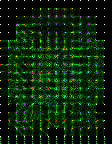
\includegraphics[scale=1.2]{images/TF/exemples_diapo_2/blason-cachan_tf_couleur.png}
		\end{tabular}
		\caption{La transformée de Fourier d'une image}
	\end{figure}
\end{frame}


%%%%%%%%%%%%%%%%%%%%%%%%%%%%%%%%%%%%%%%%%%%%%%%%
% Quatrième diapo
%%%%%%%%%%%%%%%%%%%%%%%%%%%%%%%%%%%%%%%%%%%%%%%%
\begin{frame}{La transformée de Fourier}{Comment calculer la transformée de Fourier d'une image}
	\begin{block}{Transformée de Fourier discrète}
		La transformée de Fourier est une application linéaire de \(\mathbb{C}^n$ dans $\mathbb{C}^n\)
		Soit \(X\in\mathbb{C}^n\) \\
		Le vecteur transformé s'exprime \(\widehat{X} = AX\) avec \(A = {\left(\exp\left(2\mathbf{i}\pi\frac{kl}{n}\right)\right)}_{\substack{0 \leqslant k \leqslant n-1,\\ 0 \leqslant l \leqslant n-1}}\)
	\end{block}
\end{frame}

%%%%%%%%%%%%%%%%%%%%%%%%%%%%%%%%%%%%%%%%%%%%%%%%
% Cinquième diapo
%%%%%%%%%%%%%%%%%%%%%%%%%%%%%%%%%%%%%%%%%%%%%%%%
\begin{frame}{La transformée de Fourier}{Comment calculer la transformée de Fourier d'une image}
	\begin{align*}
		{
		M = 
		\begin{pmatrix}
				x_{0,0} \dots x_{0,n-1} \\
				\vdots \phantom{x_{0} \dots x_{0}} \vdots\\ 
				x_{n-1,0} \dots x_{n-1,n-1} \\
		\end{pmatrix}
		}
		\longrightarrow
		{
		 	\begin{pmatrix}
				x_{0,0}\\
				\vdots\\
				x_{0,n-1}\\
				\vdots\\
				x_{n-1,n-1}
			\end{pmatrix}
		}
		= X
	\end{align*}
\end{frame}

%%%%%%%%%%%%%%%%%%%%%%%%%%%%%%%%%%%%%%%%%%%%%%%%
% Sixième diapo
%%%%%%%%%%%%%%%%%%%%%%%%%%%%%%%%%%%%%%%%%%%%%%%%
\begin{frame}{La transformée de Fourier}{Comment calculer la transformée de Fourier d'une image}
	\begin{block}{Algorithme naïf}
		Soit \(X \in \mathbb{C}^{n\times m}\)\\
		\begin{itemize}
			\item <2-> \(X = (x_{i,j})_{\substack{0 \leqslant k \leqslant n-1,\\ 0 \leqslant l \leqslant m-1}}\)
			\item <3-> \(A = \left(\frac{1}{\sqrt{nm}}\exp{\left(2\mathbf{i}\pi\left(\frac{ik}{n}+\frac{jl}{m}\right)\right)}\right)_{\substack{0 \leqslant i,k \leqslant n-1,\\ 0 \leqslant j,l \leqslant m-1}}\)
		\end{itemize}
		
		\onslide<4->{D'où le vecteur transformé :
		\[\widehat{X}_{i,j} = [AX]_{i,j} = \frac{1}{\sqrt{nm}}\sum_{k=0}^{n}\sum_{l=0}^{m-1} x_{k,l}e^{\left(2\mathbf{i}\pi\left(\frac{ik}{n}+\frac{kl}{m}\right)\right)}\]
		}
	\onslide<5-> On obtient donc un algorithme en \(\mathcal{O}(N^2)\) où \(N=n\times m\) est la taille de l'image.
	\end{block}
\end{frame}

%%%%%%%%%%%%%%%%%%%%%%%%%%%%%%%%%%%%%%%%%%%%%%%%
% Septième diapo
%%%%%%%%%%%%%%%%%%%%%%%%%%%%%%%%%%%%%%%%%%%%%%%%
\begin{frame}{La transformée de Fourier}{De meilleurs algorithmes}
	\begin{block}{Utiliser la séparabilité}
		\onslide<2->{On peut réécrire le calcul précédent : 
		\[\widehat{X}_{i,j} = [AX]_{i,j} = \frac{1}{\sqrt{n}}\sum_{k=0}^{n-1} e^{\left(2\mathbf{i}\pi\left(\frac{ik}{n}\right)\right)} \frac{1}{\sqrt{m}}\sum_{l=0}^{n-1} x_{k,l}e^{\left(2\mathbf{i}\pi\left(\frac{jl}{m}\right)\right)}\]
		}
		\onslide<3-> On voit apparaître deux transformations unidimensionnelles successives, sur les lignes, puis les colonnes.\\

		\onslide<4->{Dans le cas où \(n = m\), le calcul du vecteur transformé devient : 

		\[\widehat{M} = AMA^t, \textrm{où} \, A = {\left(\frac{1}{\sqrt{n}}\exp\left(2\mathbf{i}\pi\frac{kl}{n}\right)\right)}_{\substack{0 \leqslant k \leqslant n-1,\\ 0 \leqslant l \leqslant n-1}}\]
		}
		\onslide<5->On obtient finalemenent un algorithme en \(\mathcal{O}(N)\) où \(N=n\times m\) est la taille de l'image.
	\end{block}
\end{frame}	

%%%%%%%%%%%%%%%%%%%%%%%%%%%%%%%%%%%%%%%%%%%%%%%%
% Huitième diapo
%%%%%%%%%%%%%%%%%%%%%%%%%%%%%%%%%%%%%%%%%%%%%%%%
\begin{frame}{La transformée de Fourier}{La transformée en cosinus discrète}
	
	\onslide<1->{
	\begin{block}{Inconvénients de la transformée de Fourier}
		\begin{itemize}
			\item <2-> Coefficients complexes
			\item <3-> Décroissance des coefficients vers le centre de l'image \(\rightarrow\) suppression de coefficients importants :
			contradictions avec le Système Visuel Humain.
		\end{itemize}
	\end{block}
	}
	\onslide<4->{
	\begin{block}{Une solution : la transformée en cosinus discrète}
		\begin{itemize}
			\item <5-> Opération basés sur la TF donc mêmes avantages
			\item <6-> Règle les problèmes énumérés précédement
			\item <7-> Décroissance des coefficients vers les hautes fréquences \(\rightarrow\) en accord avec le Système Visuel Humain 
		\end{itemize}
	\end{block}
	}

\end{frame}

%%%%%%%%%%%%%%%%%%%%%%%%%%%%%%%%%%%%%%%%%%%%%%%%
% Neuvième diapo
%%%%%%%%%%%%%%%%%%%%%%%%%%%%%%%%%%%%%%%%%%%%%%%%
\begin{frame}{La transformée de Fourier}{Comparaison entre la TF et la TCD}
	\begin{figure}
		\begin{tabular}{ c c c}
			
\includegraphics[scale=13]{images/TF/comparaison_tf_tcd/diapo_tf_img.png} &
			
\includegraphics[scale=13]{images/TF/comparaison_tf_tcd/diapo.png} &
			
\includegraphics[scale=13]{images/TF/comparaison_tf_tcd/diapo_tcd_img.png}
		\end{tabular}
		\caption{À gauche TF; Au milieu image de base; À droite TCD}
	\end{figure}
\end{frame}